\section{Strømforsyning} %Please start me on a left page :)
\subsection{Printudlæg}

For at implementere kredsløbet i figur \ref{fig:bil_psu} på side \pageref{fig:bil_psu} er der udarbejdet et PCB layout for strømforsyningen.
Dette kan ses i figur \ref{fig:bil_psu_pcb}. 
Under udlægget af printet er der taget forbehold for at minimere arealet af strømsløjfer, som ligger i forbindelse med den skiftende udgang samt returveje derfra på LM26003. Ydermere er der også forsøgt at give så god elektrisk kontakt som muligt ved hjælp af brede printbaner til de komponenter, som forventes at trække en stor, evt. skiftende, strøm.
Dette kan ses i området omkring 3V udgangen fx, da diode, spole, udgang samt kondensator ligger helt op ad hinanden. 
De kredse, som ligger i forbindelse med tilbagekoblingen til LM26003 ligger på den 'nedre' del af printet for at minimere støjen fra de skarpe flanker på LM26003's udgang (ben 1-3 og 11-13).
Grundet at skolens komponentlager ikke lå inde med keramiske kondensatorer i størrelsen 6.8 $\mu F$ er der i stedet sat 7 parallelkoblede kondensatorer i på hver 1 $\mu F$.

Efter oplodning og test af printet blev der eftermonteret tre 2.2 $mu$F keramiske kondensatorer og forsyningen til LED'en blev skåret over for at få strømforsyningen til at give et korrekt output.
Den ene kondensator var en manglende komponent for at holde LM26003's VDD oppe under operation, da den ellers ikke kan bibeholde den spænding der skal til at for at lade bootstrap-kondensatoren opladet, denne kan ses monteret på figur \ref{fig:bil_psu_Cvdd_img}.
De øvrige kondensator er sat på som HF-afkobling ved 5V og 3V udgangen, et eksempel kan ses på figur \ref{fig:bil_psu_C5v_img}.
Grunden til at forsyningen til LED'en er kappet er at denne trak omkring 5 mA, hvilket ligger over det i databladet foreskrevne maks på 1 mA for forsyning fra VDD.
Efter ovenstående modifikationer er nedenstående tests udført.

På figur \ref{fig:bil_psu_img} ses den færdige strømforsyning.

\begin{figure}[h]
\centering
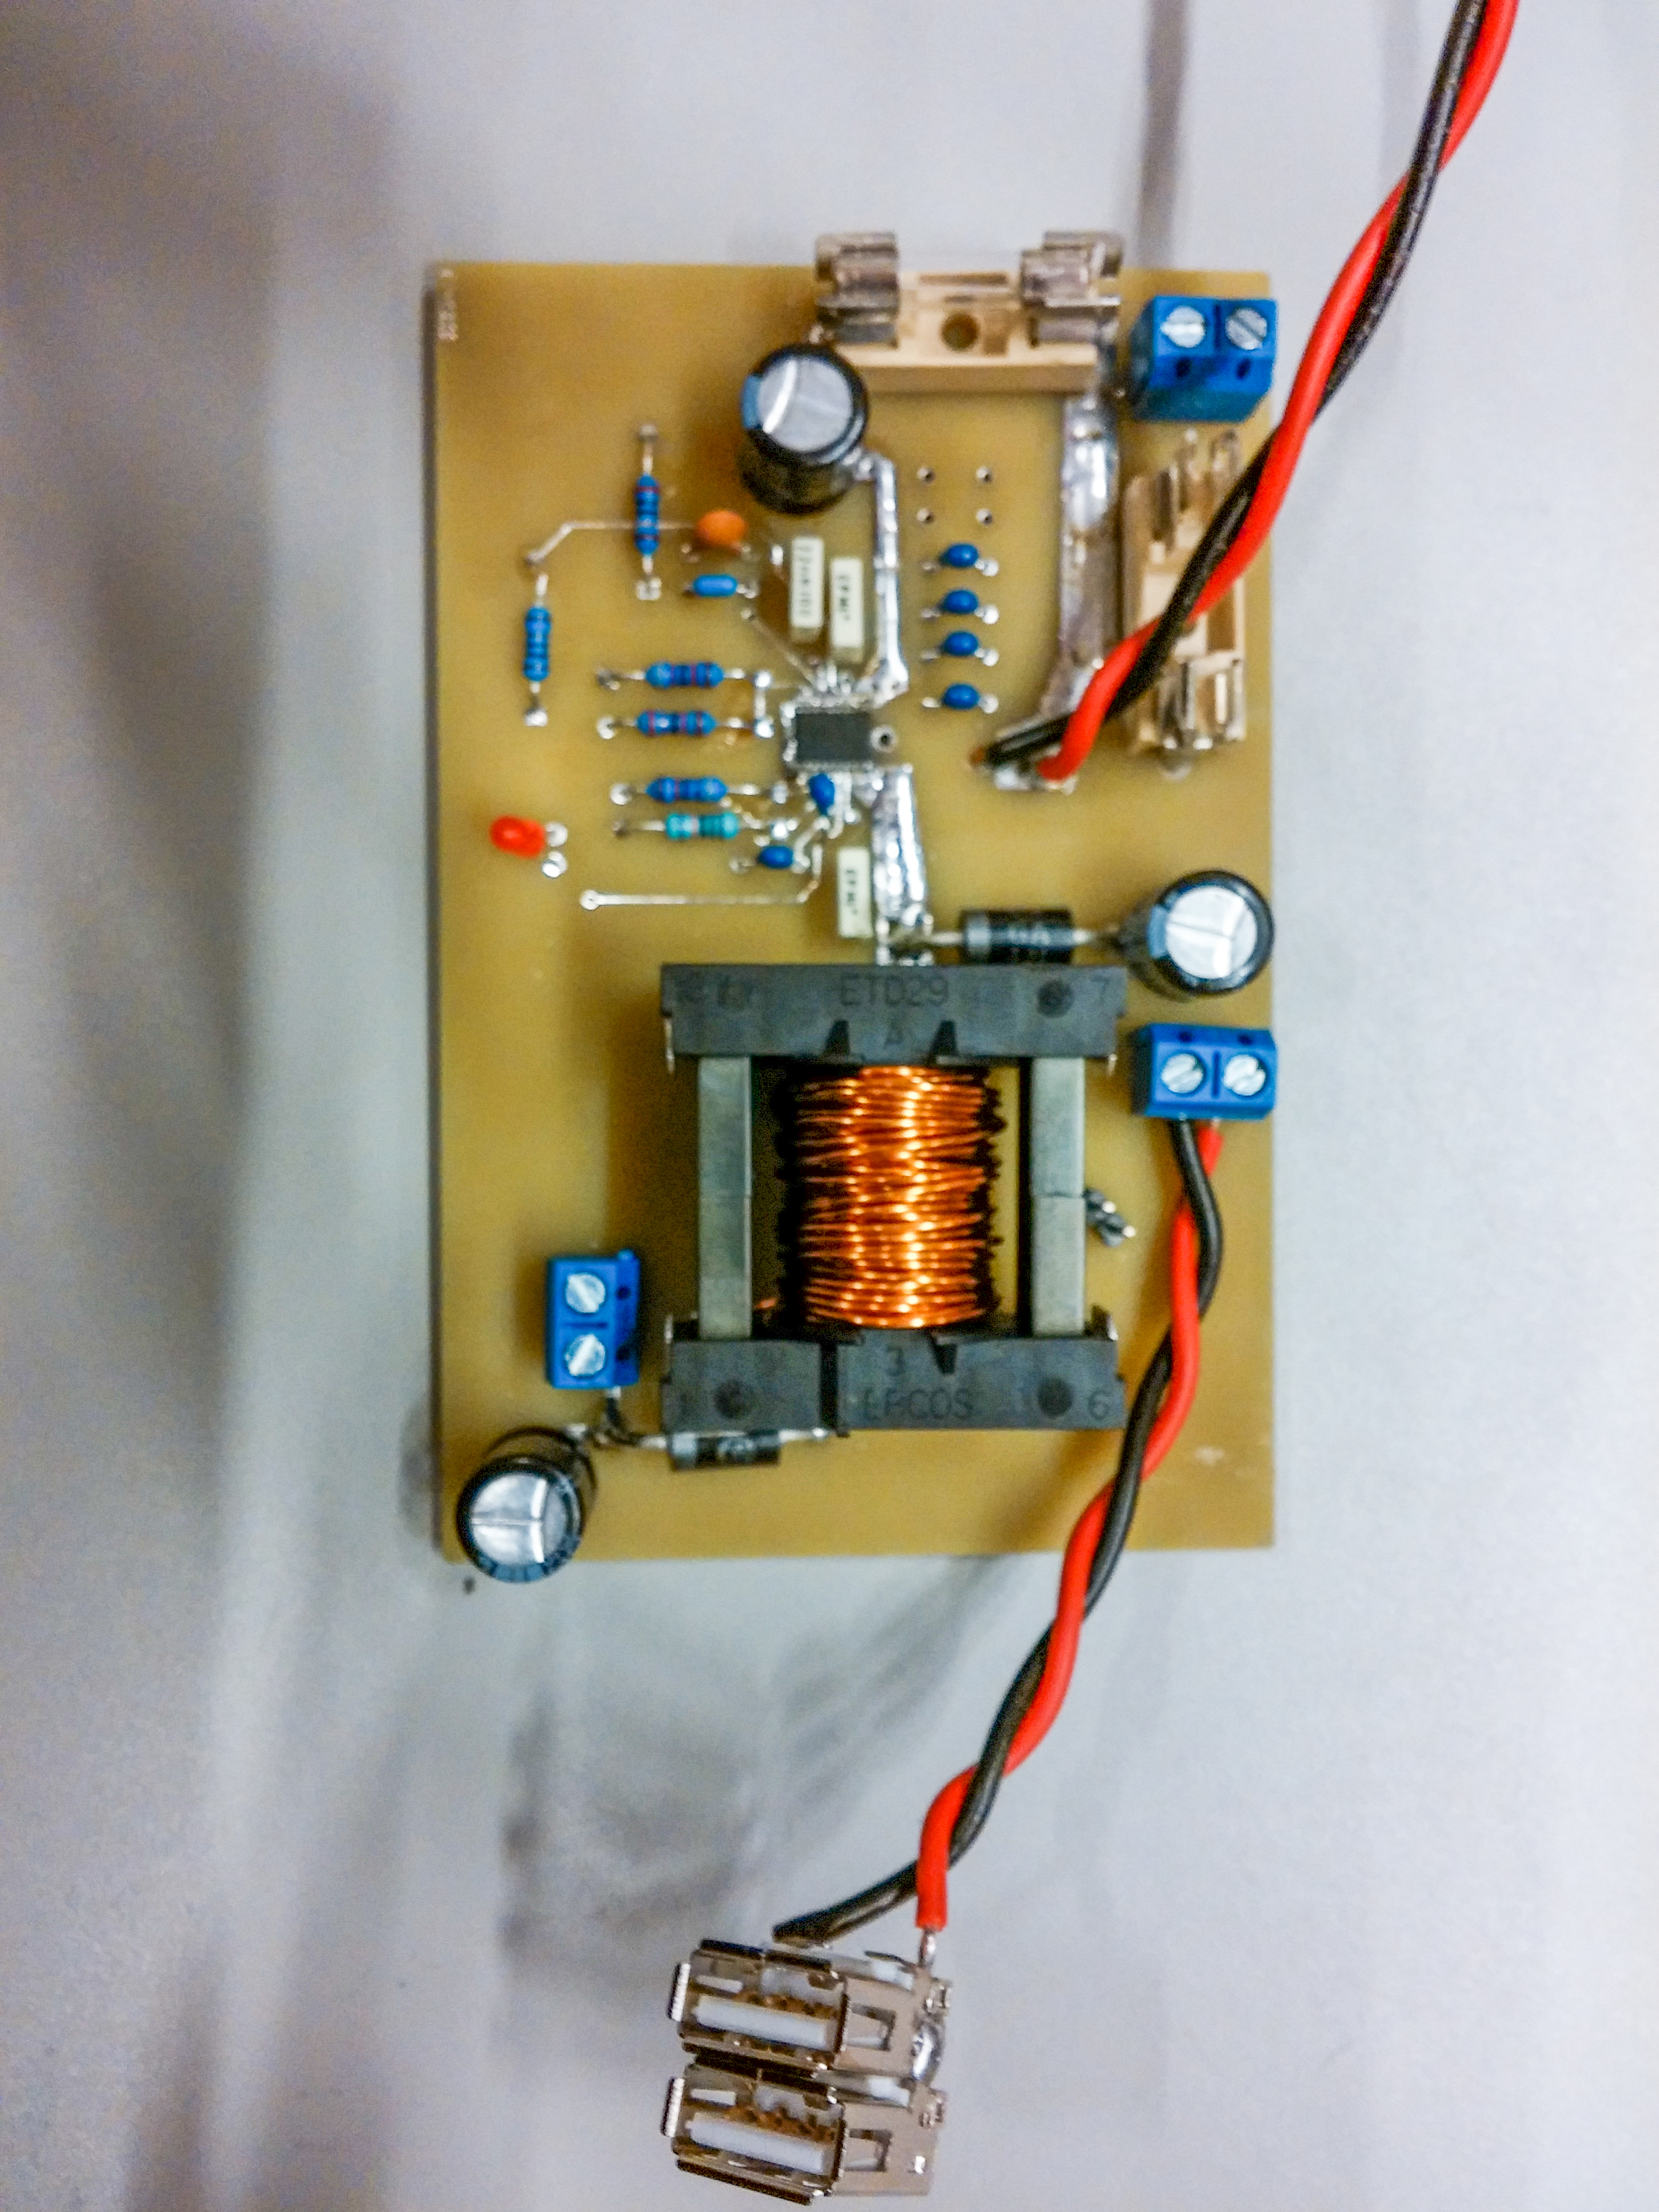
\includegraphics[angle=90, width=\textwidth- 5cm]{../fig/billeder/impl_psu/psu_pcb}
\caption{Strømforsyningen oploddet}
\label{fig:bil_psu_img}
\end{figure}

\clearpage
\begin{landscape}
\begin{figure}
\centering
\includegraphics[height=\textwidth-2cm, clip=true, trim=50 615 234 25]{../fig/diagrammer/bil/psu_pcb_twoside}
\caption{Bilens strømforsyning på PCB}
\label{fig:bil_psu_pcb}
\end{figure}
\end{landscape}

\clearpage

\begin{figure}[h]
\centering
\includegraphics[width=\textwidth- 5cm]{../fig/billeder/impl_psu/psu_vdd_konden}
\caption{Kondensator påmonteret VDD til stel}
\label{fig:bil_psu_Cvdd_img}
\end{figure}

\begin{figure}[h]
\centering
\includegraphics[width=\textwidth- 5cm]{../fig/billeder/impl_psu/psu_afkobl_konden}
\caption{Kondensator påmonteret 5V udgangen til stel}
\label{fig:bil_psu_C5v_img}
\end{figure}

\clearpage

\subsection{Test}

For at teste strømforsyningen er batteritilkoblingen på strømforsyningen koblet op mod en laboratoriespændingsforsyning indstillet til 7.2V DC med en samlet strømbegrænsning på 4A.
Strømforsyningens 5V udgang er herefter koblet i serie med et amperremeter og i parallel med et oscilloskop og et effektpotentiometer.
Effektpotentiometerets modstand er skruet ned indtil en udgangsstrøm på 2A er nået fra 5V udgangen.
Samtidigt er strømforsyningens 3V udgang koblet på til en identisk opstilling, dog med effektpotentiometeret indstillet til en udgangsstrøm på 100 mA.

Der er ved test observeret en højfrekvent lyd fra selve LM26003. 
Kikker man på figur \ref{fig:psu_test_5v} ses at spændingsripplen på udgangen har en periodetid tilsvarende 2.6 kHz, hvilket jo befinder sig indenfor det hørbare område. 
Den gennemsnitlige udgangsspænding overholder kravet om 5V $\pm$, ydermere konkluderes det at spændingsripplen dog overstiger de 1V, som forsyningen er designet ud fra kravene omkring forsyningssignaler på bilen i tabel \ref{tbl:bil_forsyninger} på side \pageref{tbl:bil_forsyninger}.

\begin{figure}[h]
\centering
\includegraphics[scale=1]{../fig/billeder/impl_psu/psu_test_5V_2A}
\caption{Oscilloskopbillede af strømforsyningens 5V udgang under test}
\label{fig:psu_test_5v}
\end{figure}

\clearpage

På figur \ref{fig:psu_test_3v} ses test af 3V udgangen under load og denne overholder ej heller helt kravene for spændingsripple på 0.2V i henhold til tabel \ref{tbl:bil_forsyninger}, dog ligger middelspændingen pænt i nærheden af 3V.

\begin{figure}[h]
\centering
\includegraphics[scale=1]{../fig/billeder/impl_psu/psu_test_3V_100mA}
\caption{Oscilloskopbillede af strømforsyningens 3V udgang under test}
\label{fig:psu_test_3v}
\end{figure}

Strømforsyningen har under accepttesten og integrationstest fungeret som primær forsyning til bilens komponenter uden problemer.